\documentclass[12pt,a4paper]{article}

\usepackage[a4paper, top=1in, bottom=1in, left=1in, right=1in, headheight=15pt]{geometry}
\usepackage{graphicx}
\usepackage{xcolor}
\usepackage{colortbl}
\usepackage{longtable}
\usepackage{array}
\usepackage{booktabs}
\usepackage{hyperref}
\usepackage{titlesec}
\usepackage{parskip}
\usepackage{enumitem}
\usepackage{fancyhdr}
\usepackage{caption}
\usepackage{float}
\usepackage{microtype}
\usepackage{tocloft}
\usepackage{needspace}
\usepackage{etoolbox}
\usepackage{tikz}
\usepackage{afterpage}
\usepackage{pdfpages}
\usepackage{xurl}
\titleformat{\section}{\large\bfseries}{}{0em}{}[\titlerule]
\titlespacing{\section}{0pt}{18pt}{8pt}
\titleformat{\subsection}{\normalsize\bfseries}{}{0em}{}
\titlespacing{\subsection}{0pt}{10pt}{4pt}

\pagestyle{fancy}
\fancyhf{}
\lhead{\small{DeenMate}}
\rhead{\small{CSE 464: Software Development Project II}}
\cfoot{\thepage}
\renewcommand{\headrulewidth}{0.5pt}

\hypersetup{colorlinks=false, pdfborder={0 0 0}}

\newcolumntype{L}[1]{>{\raggedright\arraybackslash}p{#1}}
\newcolumntype{C}[1]{>{\centering\arraybackslash}p{#1}}

\renewcommand{\cftsecfont}{\bfseries}
\renewcommand{\cftsecpagefont}{\bfseries}
\renewcommand{\cftsubsecfont}{\normalfont}
\renewcommand{\cftsubsecpagefont}{\normalfont}
\setlength{\cftbeforesecskip}{4pt}
\setlength{\cftbeforesubsecskip}{2pt}
\renewcommand{\cftsecleader}{\cftdotfill{\cftdotsep}}
\renewcommand{\cftsubsecleader}{\cftdotfill{\cftdotsep}}

\setlength{\cftfignumwidth}{2.5em}

\newenvironment{apitable}{%
  \begin{longtable}{|C{0.8cm}|C{1.6cm}|L{5.2cm}|L{5.2cm}|}
  \hline
  \rowcolor[RGB]{200,200,200}
  \textbf{No.} & \textbf{Method} & \textbf{Endpoint} & \textbf{Description} \\
  \hline
  \endfirsthead
  \endfoot
  \hline
  \endlastfoot
}{%
  \end{longtable}
}

\begin{document}

\begin{titlepage}
\thispagestyle{empty}
\centering

{\Large\bfseries MILITARY INSTITUTE OF SCIENCE AND TECHNOLOGY}

\vspace{0.45cm}

\IfFileExists{MIST Logo_0 .png}{%
  
\includegraphics[width=4cm]{MIST Logo_0 .png}%
}{%
  \fbox{\parbox[c][4cm][c]{4cm}{\centering\small MIST Logo}}%
}
 

\vspace{0.45cm}

{\large\bfseries DEPARTMENT OF COMPUTER SCIENCE AND ENGINEERING}

\vspace{0.7cm}

{\normalsize CSE 464: Software Development Project II}

\vspace{0.35cm}

{\normalsize Software Requirement Specification}

\vspace{0.2cm}

{\normalsize of}

\vspace{0.35cm}

{\Huge\bfseries DeenMate}

\vspace{0.25cm}

{\large\itshape An AI-Powered Integrated Islamic Lifestyle \& Wealth Management Platform}

\vspace{0.9cm}

{\large\bfseries Group: 10}\\[0.15cm]
{\large\bfseries Section: B}

\vspace{1.1cm}

\begin{minipage}[t]{0.46\textwidth}
\raggedright
\textbf{Submitted By}\\[0.4cm]
\begin{tabular}{@{}ll@{}}
Tasmia Nasir        & 202214108 \\[2pt]
Maria Sultana Joly  & 202314103 \\[2pt]
Afia Fahmidha Zaman & 202314106 \\[2pt]
Akhi Alam           & 202314122 \\
\end{tabular}
\end{minipage}
\hfill
\begin{minipage}[t]{0.46\textwidth}
\raggedright
\textbf{Submitted To}\\[0.4cm]
Lt Col Md Abul Basar\\[2pt]
Prof. Dr. Md Mahbubur Rahman\\[2pt]
Asso. Prof. Dr. T M Shahriar Sazzad\\[2pt]
Lec Nafisa Maliyat\\[2pt]
\end{minipage}

\vfill

{\normalsize Submission Date: June 30, 2026}
\end{titlepage}

\tableofcontents
\newpage

\section{Problem Statement}

Muslims often rely on multiple mobile applications to manage prayer schedules, Zakat calculation, Islamic inheritance, halal food verification, and Hajj/Umrah guidance. This fragmentation makes it difficult to efficiently manage religious obligations and financial planning. Existing applications usually focus on specific functionalities and lack an integrated platform that combines Islamic wealth management, worship assistance, AI-powered recommendations, and pilgrimage support. Therefore, there is a need for a secure, intelligent, and centralized Islamic lifestyle management system.

\section{Project Objectives}

\begin{enumerate}[leftmargin=2em, label=\arabic*.]
  \item To develop an integrated Islamic lifestyle management platform that provides essential religious, financial, and worship-related services in one application. 
  \item To assist users in managing their daily Islamic practices through personalized guidance, reminders, and AI-powered recommendations. 
  \item To simplify Islamic financial planning and pilgrimage preparation by providing accurate tools and user-friendly assistance. 
  \item To enhance the overall user experience by offering a secure, accessible, and intelligent mobile application for everyday Islamic needs.
\end{enumerate}

\section{Finalized Features}

\subsection*{1. User Registration \& Profile Management}
\begin{itemize}[leftmargin=2em, label=\textbullet, itemsep=3pt]
  \item Secure user registration and login.
  \item User profile management.
  \item Fiqh preference selection (Hanafi/Shafi'i).
  \item Multi-language support (English, Bengali).
\end{itemize}

\subsection*{2. Islamic Wealth Management}
\begin{itemize}[leftmargin=2em, label=\textbullet, itemsep=3pt]
  \item Zakat Calculator with Nisab checking.
  \item Qurbani \& Aqiqah guidance.
  \item Hajj \& Umrah financial planner.
  \item Islamic inheritance calculator (Al-Fara'id).
  \item Downloadable PDF financial reports.
\end{itemize}

\subsection*{3. Prayer \& Worship Management}
\begin{itemize}[leftmargin=2em, label=\textbullet, itemsep=3pt]
  \item GPS-based prayer times and Athan reminders.
  \item Hijri calendar with Islamic event notifications.
  \item Salah, Quran, and Dhikr tracking.
\end{itemize}

\subsection*{4. AI Islamic Assistant}
\begin{itemize}[leftmargin=2em, label=\textbullet, itemsep=3pt]
  \item AI-powered Islamic question answering.
  \item Personalized book, Hadith, Dua, and Surah recommendations.
  \item Personalized Islamic learning suggestions.
\end{itemize}

\subsection*{5. Hajj \& Umrah Companion}
\begin{itemize}[leftmargin=2em, label=\textbullet, itemsep=3pt]
  \item Step-by-step pilgrimage guidance.
  \item Day-wise Hajj and Umrah checklist.
  \item Live location tracking using Google Maps.
  \item Group safety and emergency alert system.
\end{itemize}

\subsection*{6. Halal Food Detection}
\begin{itemize}[leftmargin=2em, label=\textbullet, itemsep=3pt]
  \item Barcode and image-based food scanning.
  \item Halal/Haram ingredient identification.
  \item Nearby Halal restaurant finder.
\end{itemize}

\subsection*{7. Security \& Privacy}
\begin{itemize}[leftmargin=2em, label=\textbullet, itemsep=3pt]
  \item Secure financial data storage.
  \item Privacy-controlled location sharing.
  \item Family tracking consent management.
  \item Cloud backup support.
\end{itemize}

\subsection*{8. Additional Features}
\begin{itemize}[leftmargin=2em, label=\textbullet, itemsep=3pt]
  \item PDF report generation.
  \item User-friendly interface.
\end{itemize}

\clearpage
\section{ER Diagram}

\begin{figure}[H]
  \centering
  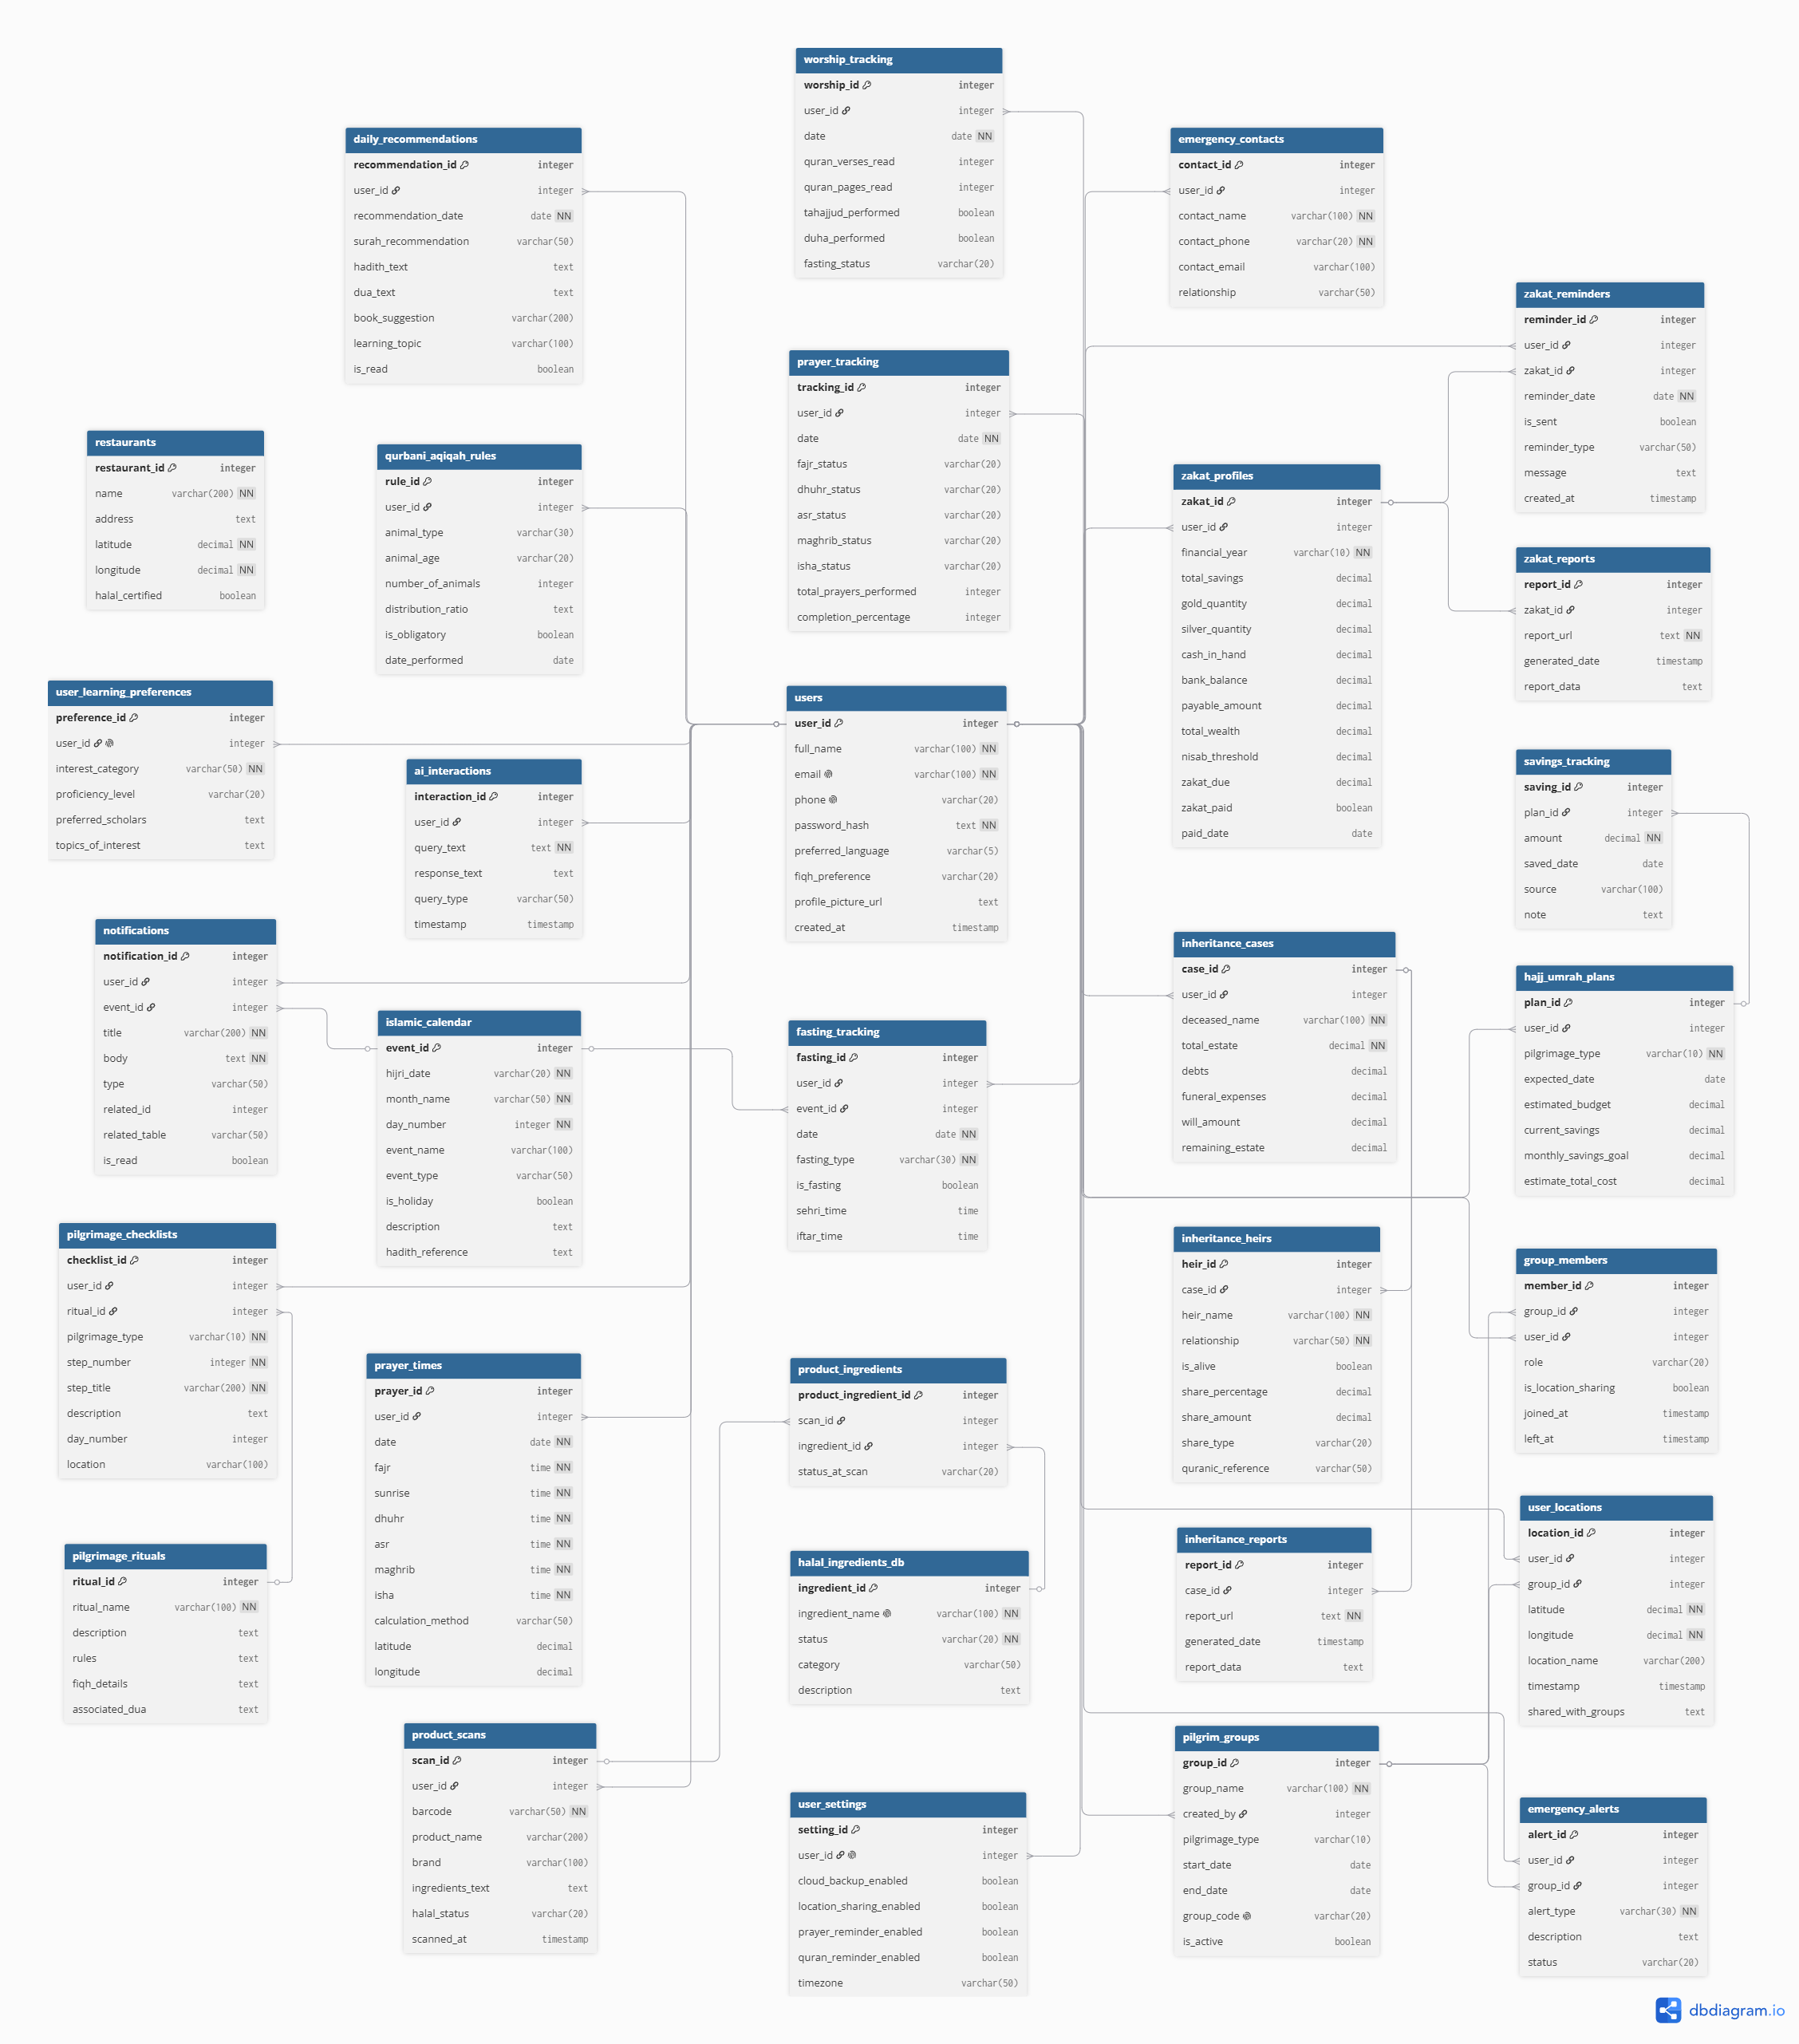
\includegraphics[page=1, width=\textwidth, keepaspectratio]{Untitled (1).png}
  \caption{Entity-Relationship Diagram for DeenMate}
  \label{fig:erd}
\end{figure}

\clearpage

\section{Tentative UI Pages}

\begin{itemize}[leftmargin=2em, label=\textbullet, itemsep=4pt]
  \item \textbf{Splash / Login / Register:} App launch screen with authentication flows --- login, signup, OTP verification, and forgot password.

  \item \textbf{Dashboard:} Home screen displaying prayer times, daily recommendations (Surah/Hadith/Dua), fasting status, and quick action buttons.

  \item \textbf{Prayer \& Worship Hub:} Combined page for prayer tracking, worship logging (Quran, Tahajjud, Duha), dhikr counter, and fasting tracker.

  \item \textbf{Islamic Calendar:} View Hijri calendar with Islamic events, holidays, and daily content.

  \item \textbf{User Profile \& Settings:} View and edit profile, manage app preferences (notifications, timezone, language), and access reports.

  \item \textbf{Notifications:} List of all app notifications with read/unread status indicators.

  \item \textbf{Halal Scanner:} Scan barcodes to check Halal status, view scan history, search individual ingredients, and find nearby Halal restaurants.

  \item \textbf{AI Islamic Assistant:} Chat interface for Islamic guidance, Fiqh queries, Tafsir, and Duas with persistent chat history.

  \item \textbf{Hajj/Umrah Planner:} Manage pilgrimage plans with budget tracking, savings goals, interactive checklists, and ritual guides.

  \item \textbf{Pilgrim Groups:} Create and manage groups for Hajj/Umrah with real-time location sharing and group coordination.

  \item \textbf{Zakat Management:} Complete Zakat module with profile setup, asset management, auto-calculation, payment tracking, reminders, and PDF report generation.

  \item \textbf{Qurbani/Aqiqah Planner:} Plan and track sacrificial offerings with Islamic rules, animal details, and scheduling.

  \item \textbf{Inheritance Calculator:} Create inheritance cases, view Islamic distribution shares, and generate downloadable PDF reports.

  \item \textbf{Safety and Security:} Manage emergency contacts, send SOS alerts with live location, and track group member locations.
\end{itemize}
\newpage

\section{Tentative APIs}

\needspace{6\baselineskip}
\subsection*{Authentication APIs}
\begin{apitable}
1 & POST & /auth/login              & User login \\                    \hline
2 & POST & /auth/register           & Register new user \\             \hline
3 & POST & /auth/verify-otp         & Verify email/phone OTP \\        \hline
4 & POST & /auth/forgot-password    & Request password reset \\        \hline
\end{apitable}

\needspace{6\baselineskip}
\subsection*{User APIs}
\begin{apitable}
5 & GET & /users/profile    & Get user profile \\     \hline
6 & PUT & /users/profile    & Update user profile \\  \hline
7 & GET & /users/settings   & Get user settings \\    \hline
8 & PUT & /users/settings   & Update user settings \\ \hline
\end{apitable}

\needspace{8\baselineskip}
\subsection*{Prayer \& Worship APIs}
\begin{apitable}
9  & GET  & /prayer/today         & Get today's prayer times \\          \hline
10 & GET  & /prayer/tracking      & Get prayer tracking for date \\       \hline
11 & POST & /prayer/tracking      & Update prayer status \\               \hline
12 & POST & /worship/tracking     & Log worship activities \\             \hline
13 & POST & /dhikr/tracking       & Log dhikr count \\                    \hline
14 & GET  & /fasting/today        & Get fasting status \\                 \hline
15 & POST & /fasting/tracking     & Log fasting status \\                 \hline
\end{apitable}

\needspace{6\baselineskip}
\subsection*{Calendar \& Content APIs}
\begin{apitable}
16 & GET & /calendar/month          & Get Islamic calendar events \\ \hline
17 & GET & /recommendations/daily   & Get daily content \\           \hline
\end{apitable}

\needspace{6\baselineskip}
\subsection*{Notification APIs}
\begin{apitable}
18 & GET & /notifications              & Get all notifications \\        \hline
19 & PUT & /notifications/\{id\}/read  & Mark notification as read \\    \hline
\end{apitable}

\needspace{6\baselineskip}
\subsection*{Halal Scanner APIs}
\begin{apitable}
20 & POST & /halal/scan                   & Scan product barcode \\        \hline
21 & GET  & /halal/ingredient/\{name\}    & Check ingredient status \\     \hline
\end{apitable}

\needspace{6\baselineskip}
\subsection*{AI Assistant APIs}
\begin{apitable}
22 & POST & /ai/chat                  & Send query to AI assistant \\   \hline
23 & GET  & /learning/preferences     & Get learning preferences \\     \hline
24 & POST & /learning/preferences     & Set learning preferences \\     \hline
\end{apitable}

\needspace{12\baselineskip}
\subsection*{Hajj/Umrah APIs}
\begin{apitable}
25 & GET  & /pilgrimage/plans                    & Get all pilgrimage plans \\        \hline
26 & POST & /pilgrimage/plans                    & Create pilgrimage plan \\          \hline
27 & PUT  & /pilgrimage/plans/\{id\}             & Update pilgrimage plan \\          \hline
28 & GET  & /pilgrimage/checklists               & Get pilgrimage checklists \\       \hline
29 & PUT  & /pilgrimage/checklists/\{id\}        & Mark checklist step complete \\    \hline
30 & GET  & /pilgrimage/groups                   & Get pilgrimage groups \\           \hline
31 & POST & /pilgrimage/groups                   & Create pilgrimage group \\         \hline
32 & POST & \url{/pilgrimage/groups/\{id\}/members} & Add member to group \\ \hline
33 & POST & /pilgrimage/location                 & Share live location \\             \hline
\end{apitable}

\needspace{10\baselineskip}
\subsection*{Zakat APIs}
\begin{apitable}
34 & GET  & /zakat/profile        & Get zakat profile \\           \hline
35 & POST & /zakat/profile        & Create/update zakat profile \\ \hline
36 & GET  & /zakat/assets         & Get zakat assets \\            \hline
37 & POST & /zakat/assets         & Add zakat asset \\             \hline
38 & GET  & /zakat/calculation    & Calculate zakat due \\         \hline
39 & POST & /zakat/pay            & Mark zakat as paid \\          \hline
\end{apitable}

\needspace{6\baselineskip}
\subsection*{Qurbani APIs}
\begin{apitable}
40 & GET  & /qurbani/plans    & Get Qurbani/Aqiqah plans \\      \hline
41 & POST & /qurbani/plans    & Create Qurbani/Aqiqah plan \\    \hline
42 & GET  & /qurbani/rules    & Get sacrificial rules \\          \hline
\end{apitable}

\needspace{8\baselineskip}
\subsection*{Inheritance APIs}
\begin{apitable}
43 & POST & /inheritance/cases              & Create inheritance case \\       \hline
44 & GET  & /inheritance/cases              & Get all inheritance cases \\     \hline
45 & GET  & /inheritance/cases/\{id\}       & Get case details \\              \hline
46 & GET  & \url{/inheritance/cases/{id}/report} & Generate inheritance report \\  \hline
\end{apitable}

\needspace{6\baselineskip}
\subsection*{Emergency APIs}
\begin{apitable}
47 & GET  & /emergency/contacts   & Get emergency contacts \\  \hline
48 & POST & /emergency/contacts   & Add emergency contact \\   \hline
49 & POST & /emergency/alerts     & Send SOS alert \\          \hline
\end{apitable}

\needspace{6\baselineskip}
\subsection*{PDF Reports APIs}
\begin{apitable}
50 & POST & /reports/generate         & Generate PDF report \\   \hline
51 & GET  & /reports                  & Get all reports \\       \hline
52 & GET  & /reports/\{id\}/download  & Download PDF report \\   \hline
\end{apitable}

\section{App Review}

\begin{longtable}{|L{2.6cm}|L{5.6cm}|L{5.6cm}|}
\hline
\rowcolor[RGB]{200,200,200}
\textbf{Application} & \textbf{Features} & \textbf{Limitations} \\
\hline
\endfirsthead
\endfoot
\hline
\endlastfoot
\textbf{Muslim Pro} &
\begin{itemize}
\item Prayer times \& Athan
\item Quran with audio
\item Qibla compass
\item Islamic calendar
\item Zakat calculator
\item Halal restaurant finder
\end{itemize}
&
\begin{itemize}
\item No inheritance calculator
\item No Qurbani \& Aqiqah guidance
\item No AI-powered assistant
\item No Hajj safety features
\end{itemize}
\\ \hline
\textbf{Athan} &
\begin{itemize}
\item Prayer times
\item Quran
\item Qibla direction
\item Mosque finder
\item Duas \& Dhikr
\end{itemize}
&
\begin{itemize}
\item No Islamic wealth management
\item No inheritance calculator
\item No AI assistant
\item No pilgrimage planning
\end{itemize}
\\ \hline
\textbf{Quran Majeed} &
\begin{itemize}
\item Quran with translations
\item Audio recitation
\item Tafsir
\item Prayer times
\item Qibla compass
\end{itemize}
&
\begin{itemize}
\item Focuses mainly on Quran learning
\item No Zakat management
\item No AI recommendations
\item No Hajj companion features
\end{itemize}
\\ \hline
\textbf{Quranly} &
\begin{itemize}
\item Daily Quran planner
\item Reading streaks
\item Progress tracking
\item Reading reminders
\end{itemize}
&
\begin{itemize}
\item Only Quran-focused
\item No prayer management
\item No financial tools
\item No Halal food detection
\end{itemize}
\\ \hline
\end{longtable}

\subsection*{Research Gap}

Existing Islamic applications primarily focus on prayer management and Islamic learning. While some applications provide Zakat calculation , none offer a comprehensive platform integrating Islamic wealth management (Zakat, Nisab monitoring, inheritance, Qurbani, and Aqiqah), AI-powered Islamic recommendations, Hajj \& Umrah financial planning, live pilgrimage safety, and halal food verification within a single application. To addresses these limitations by providing an all-in-one AI-powered Islamic lifestyle and wealth management system.

\section{Contribution Table}

\begin{longtable}{|L{3.8cm}|C{2.6cm}|L{6.4cm}|}
\hline
\rowcolor[RGB]{200,200,200}
\textbf{Member} & \textbf{ID} & \textbf{Contributions} \\
\hline
\endfirsthead
\endfoot
\hline
\endlastfoot
Tasmia Nasir        & 202214108 & Tentative APIs \\ \hline
Maria Sultana Joly  & 202314103 & ER Diagram \\ \hline
Afia Fahmidha Zaman & 202314106 & Problem Statement, Project Objectives, Finalized Features, App Review  \\ \hline
Akhi Alam           & 202314122 & Tentative UI Pages \\ \hline
\end{longtable}

\end{document}
